\section{Results II: the small language model is supervision-bound}\label{sec:lang}

\subsection{What the interface costs}

The same \LlmRows{} held-out transactions (\LlmPositives{} positives) are scored
twice by the same \num{0.5}-billion-parameter instruction-tuned model
\cite{qwen2024report}, once through the logit interface and once through generated
JSON. Reading the answer as a probability costs \LlmMsRow\,ms per row
(\LlmRowsPerS{} rows/s); generating and parsing a JSON object costs
\JsonMsRow\,ms per row (\JsonRowsPerS{} rows/s). The interface alone accounts for
a factor of \InterfaceRatio{} in latency, more than the difference between the two
model sizes we measure in Section~\ref{sec:scale} and more than most architecture
choices a practitioner would deliberate over. The cost sits in the interface, not
in the model.

The JSON interface also fails, completely. All \ParseFailRows{} of
\ParseFailDenom{} attempts were unparsable, and the failures are not random: the
model answered conversationally, with the same preamble every time, for example
``\emph{No. This transaction appears to be legitimate, as it includes all required
fields \dots}''. Every failure therefore maps to the same constant, the score
distribution collapses to a single value, and any ranking metric computed on the
imputed fallback would be measuring the fallback rather than the model. The
original pipeline of this project did exactly that, substituting $0.9$ or $0.1$
depending on the surface form of the failure. We record the failures and report
them; the discrimination numbers below use the logit interface, which has nothing
to parse.

\subsection{Zero-shot discrimination}

\begin{table}[t]
\centering
\resizebox{\textwidth}{!}{\begin{tabular}{lrrrrrr}
\toprule
system & AUC-PR & AUC-ROC & R@FPR$=1\%$ & F1 & parse fail & ms/row \\
\midrule
GBDT, same rows & 0.5295 & 0.9053 & 35.5\% & 0.4356 & -- & -- \\
0.5B, logit interface & 0.0767 & 0.6412 & 4.8\% & 0.0750 & 100.0\% & 6.3 \\
0.5B, JSON interface & -- & -- & -- & -- & 100.0\% & 139.5 \\
0.5B + LoRA (900 rows) & 0.0364 & 0.4582 & 0.0\% & 0.0000 & 0.0\% & 7.8 \\
\bottomrule
\end{tabular}
}
\caption{Language model against gradient-boosted trees on identical held-out rows.
The logit interface reads $P(\texttt{Yes})$ at the answer position; the JSON
interface generates and parses an object. Parse failures are counted, never
imputed. Latency is per row in the same run. Data:
\texttt{s8\_llm/zero\_shot\_0\_5b.json},
\texttt{s8\_llm/lora\_sft\_0\_5b.json}.}
\label{tab:llm}
\end{table}

Table~\ref{tab:llm} reports the comparison. The model is not at chance: AUC-ROC
\LlmAucRoc{} and AUC-PR \LlmAucPr{} against a base rate of
$\LlmPositives/\LlmRows\approx 4.1\%$ show that it extracts some signal from the
serialised row. But the gradient-boosted model on the same rows reaches AUC-PR
\GbdtSameAucPr{} and AUC-ROC \GbdtSameAucRoc{}, and the paired difference is
\LlmDelta{} with a row-level bootstrap interval of
\LlmCiLo--\LlmCiHi{} and a permutation $p<10^{-3}$. At the auditable operating
point, recall at a $1\%$ false-positive rate, the gap is
\LlmRecall\% against \GbdtSameRecall\%. The claim that a locally hosted model of
this size comes within two points of the tabular baseline is therefore refuted at
this scale, and the artefact records the corresponding flag as false.

\begin{figure}[t]
\centering
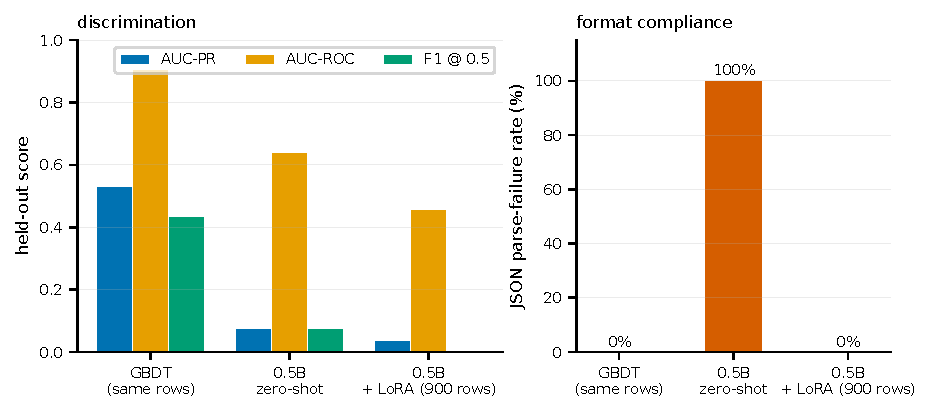
\includegraphics[width=\textwidth]{fig5_llm.pdf}
\caption{Left: held-out AUC-PR, AUC-ROC and $F_1$ for the tabular baseline and two
variants of the language model. Right: rate of unparsable JSON answers. Adaptation
moves the right panel from complete failure to complete success while moving the
left panel in the wrong direction. Data: \texttt{s8\_llm/*.json}.}
\label{fig:llm}
\end{figure}

\subsection{Adaptation repairs the format and destroys the discrimination}

LoRA \cite{hu2022lora} is applied to the query, key, value and output projections
($r=8$), giving \SftTrainable{} trainable parameters, \SftTrainablePct\% of the
model. The training set is \SftRows{} rows with per-row continuous targets: the
supervised baseline's predicted probability for that row, with mean \TargetMean,
standard deviation \TargetSd{} and \TargetDistinct{} distinct values in
$[\TargetMin,\TargetMax]$. The target therefore carries the difficulty of each row
instead of a constant. Training
takes \SftSeconds\,s on the same device, reaching a loss of \SftLoss{} with
\SftVram\,GiB peak memory.

The result is a clean dissociation, and it is the sharpest evidence in this paper
(Table~\ref{tab:llm}, right-hand rows, and Figure~\ref{fig:llm}). The parse-failure
rate goes from \ParseFailZero\% to \SftParseFail\%: adaptation teaches the output
convention perfectly. At the same time AUC-PR falls from \LlmAucPr{} to
\SftAucPr{} ($\Delta=\SftDelta$) and AUC-ROC falls from \LlmAucRoc{} to
\SftAucRoc, i.e. to chance; $F_1$ at a $0.5$ threshold goes to \SftFOne{} because
the adapted model stops emitting positive answers altogether.

We read this as an identification rather than a curiosity. Two properties of the
system used to change together, format compliance and decision quality, and the
literature on prompting and adaptation usually reports them as one number. By
measuring them separately we can say which one the update moved. \SftRows{}
labelled rows are enough to teach a syntax and not enough to teach a boundary; the
degradation is therefore evidence about supervision, not about the adaptation
method, which did exactly what it was asked. The corollary for practice is
uncomfortable: with a small labelled set, an adapted language model can look
\emph{more} usable (it answers in the requested format) while being \emph{less}
useful (it ranks worse than the prompt it replaced).

\subsection{Two model sizes, and why we stop there}\label{sec:scale}

We measure a second size, \LargeParams{}B parameters, on a \ScaleRows-row subset:
\LargeVram\,GiB peak memory and AUC-PR \LargeAucPr, against \SmallVram\,GiB and
\SmallAucPr{} for the \SmallParams{}B model. The larger model is not better on this
task; with two points we cannot distinguish a genuine inverse-scaling effect from
noise in a \ScaleRows-row evaluation, and we do not try. What the two points do support
is a memory statement: peak memory grows at \ScaleSlope\,GiB per billion
parameters, so a $7$B model at this precision would need roughly four times the
\GpuMemGiB\,GiB of the device under test. Extrapolating further would be a model of
our own making, not a measurement, and the artefact labels it as a two-point fit.
The scale question a reviewer will ask, whether the gap closes at $7$B or $8$B,
is left open, with the command that would answer it in \ref{app:artifact}.

\subsection{Verdict}

H7 holds. A half-billion-parameter model is an order of magnitude behind
gradient-boosted trees in AUC-PR on identical rows, its interface choice costs a
factor of \InterfaceRatio{} in latency, its generative interface fails on every
row, and adaptation on $10^2$ rows moves the format and the discrimination in
opposite directions. None of this says that language models cannot make tabular
decisions; it says that at this size and this supervision budget the substitution
is not neutral, and that the two failure modes must be measured separately to see
which one is binding.
